\chapter{METODOLOGIA}\label{chap:metodologia}

Este trabalho possui pesquisa aplicada\ldots

Utilizamos programação em linguagem C para sistema Linux, com metologia de desenvolvimento em código aberto\ldots

Utilizamos, inicialmente, um sensor inercial modelo MPU-6050 (Figura~\ref{fig:mpu6050-sensor-top}) anexado a uma Raspberry Pi 3B (Figuras~\ref{fig:mpu6050-proto-top}~e~\ref{fig:mpu6050-proto-top}):
\begin{figure}[H]
    \centering
    \caption{Sensor MPU-6050 encapsulado}\label{fig:mpu6050-sensor-top}
    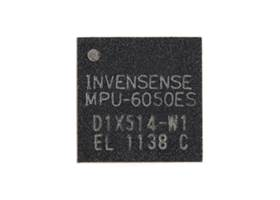
\includegraphics[width=0.5\textwidth]{figuras/mpu6050-sensor-top-straight.jpg}
    \fonte{o autor}
\end{figure}
A orientação dos sensores em relação ao encapsulamento obedece a regra da mão direita, conforme descrito na Figura~\ref{fig:mpu6050-diagram-axis}:
\begin{figure}[H]
    \centering
    \caption{Eixos do sensor em relação ao encapsulamento}\label{fig:mpu6050-diagram-axis}
    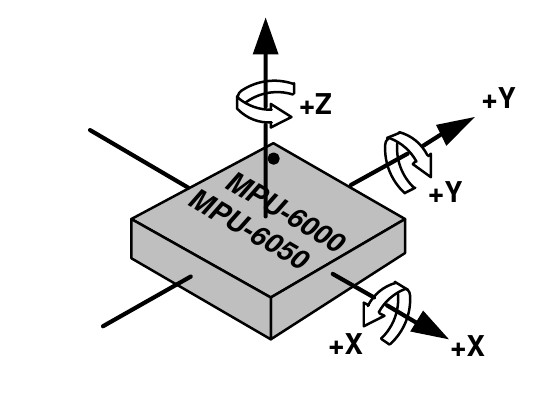
\includegraphics[width=0.5\textwidth]{figuras/mpu6050-diagram-axis.jpg}
    \fonte{\citeonline{mpu6050ps}}
\end{figure}
\begin{figure}[H]
    \centering
    \caption{Sensor MPU-6050 montado em placa módulo}\label{fig:mpu6050-board-top}
    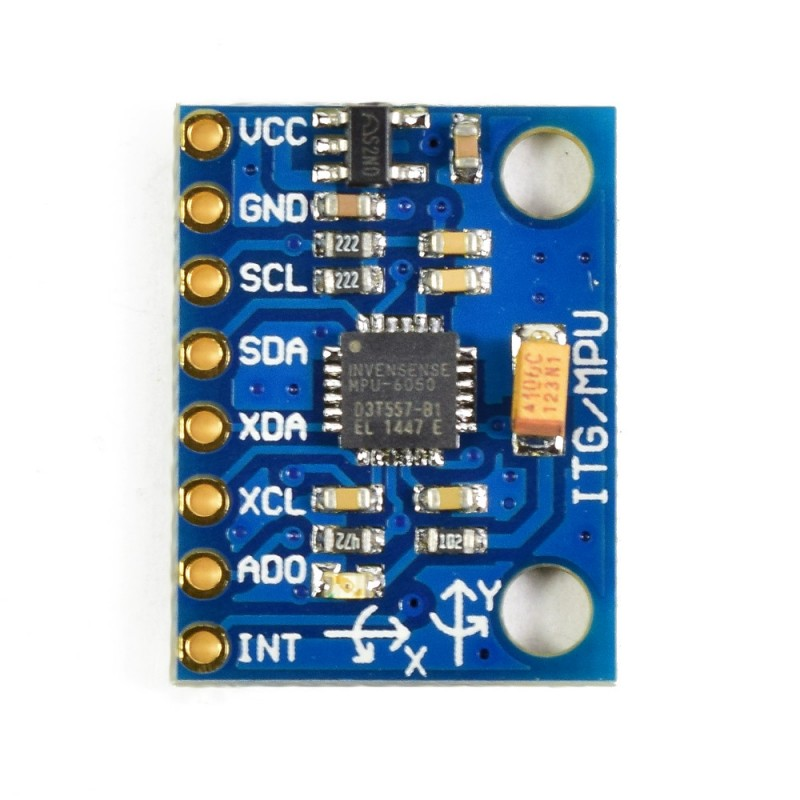
\includegraphics[width=0.5\textwidth]{figuras/mpu6050-board-top.jpg}
    \fonte{o autor}
\end{figure}
\begin{figure}[H]
    \centering
    \caption{Sensor MPU-6050 anexado à Raspberry Pi}\label{fig:mpu6050-proto-top}
    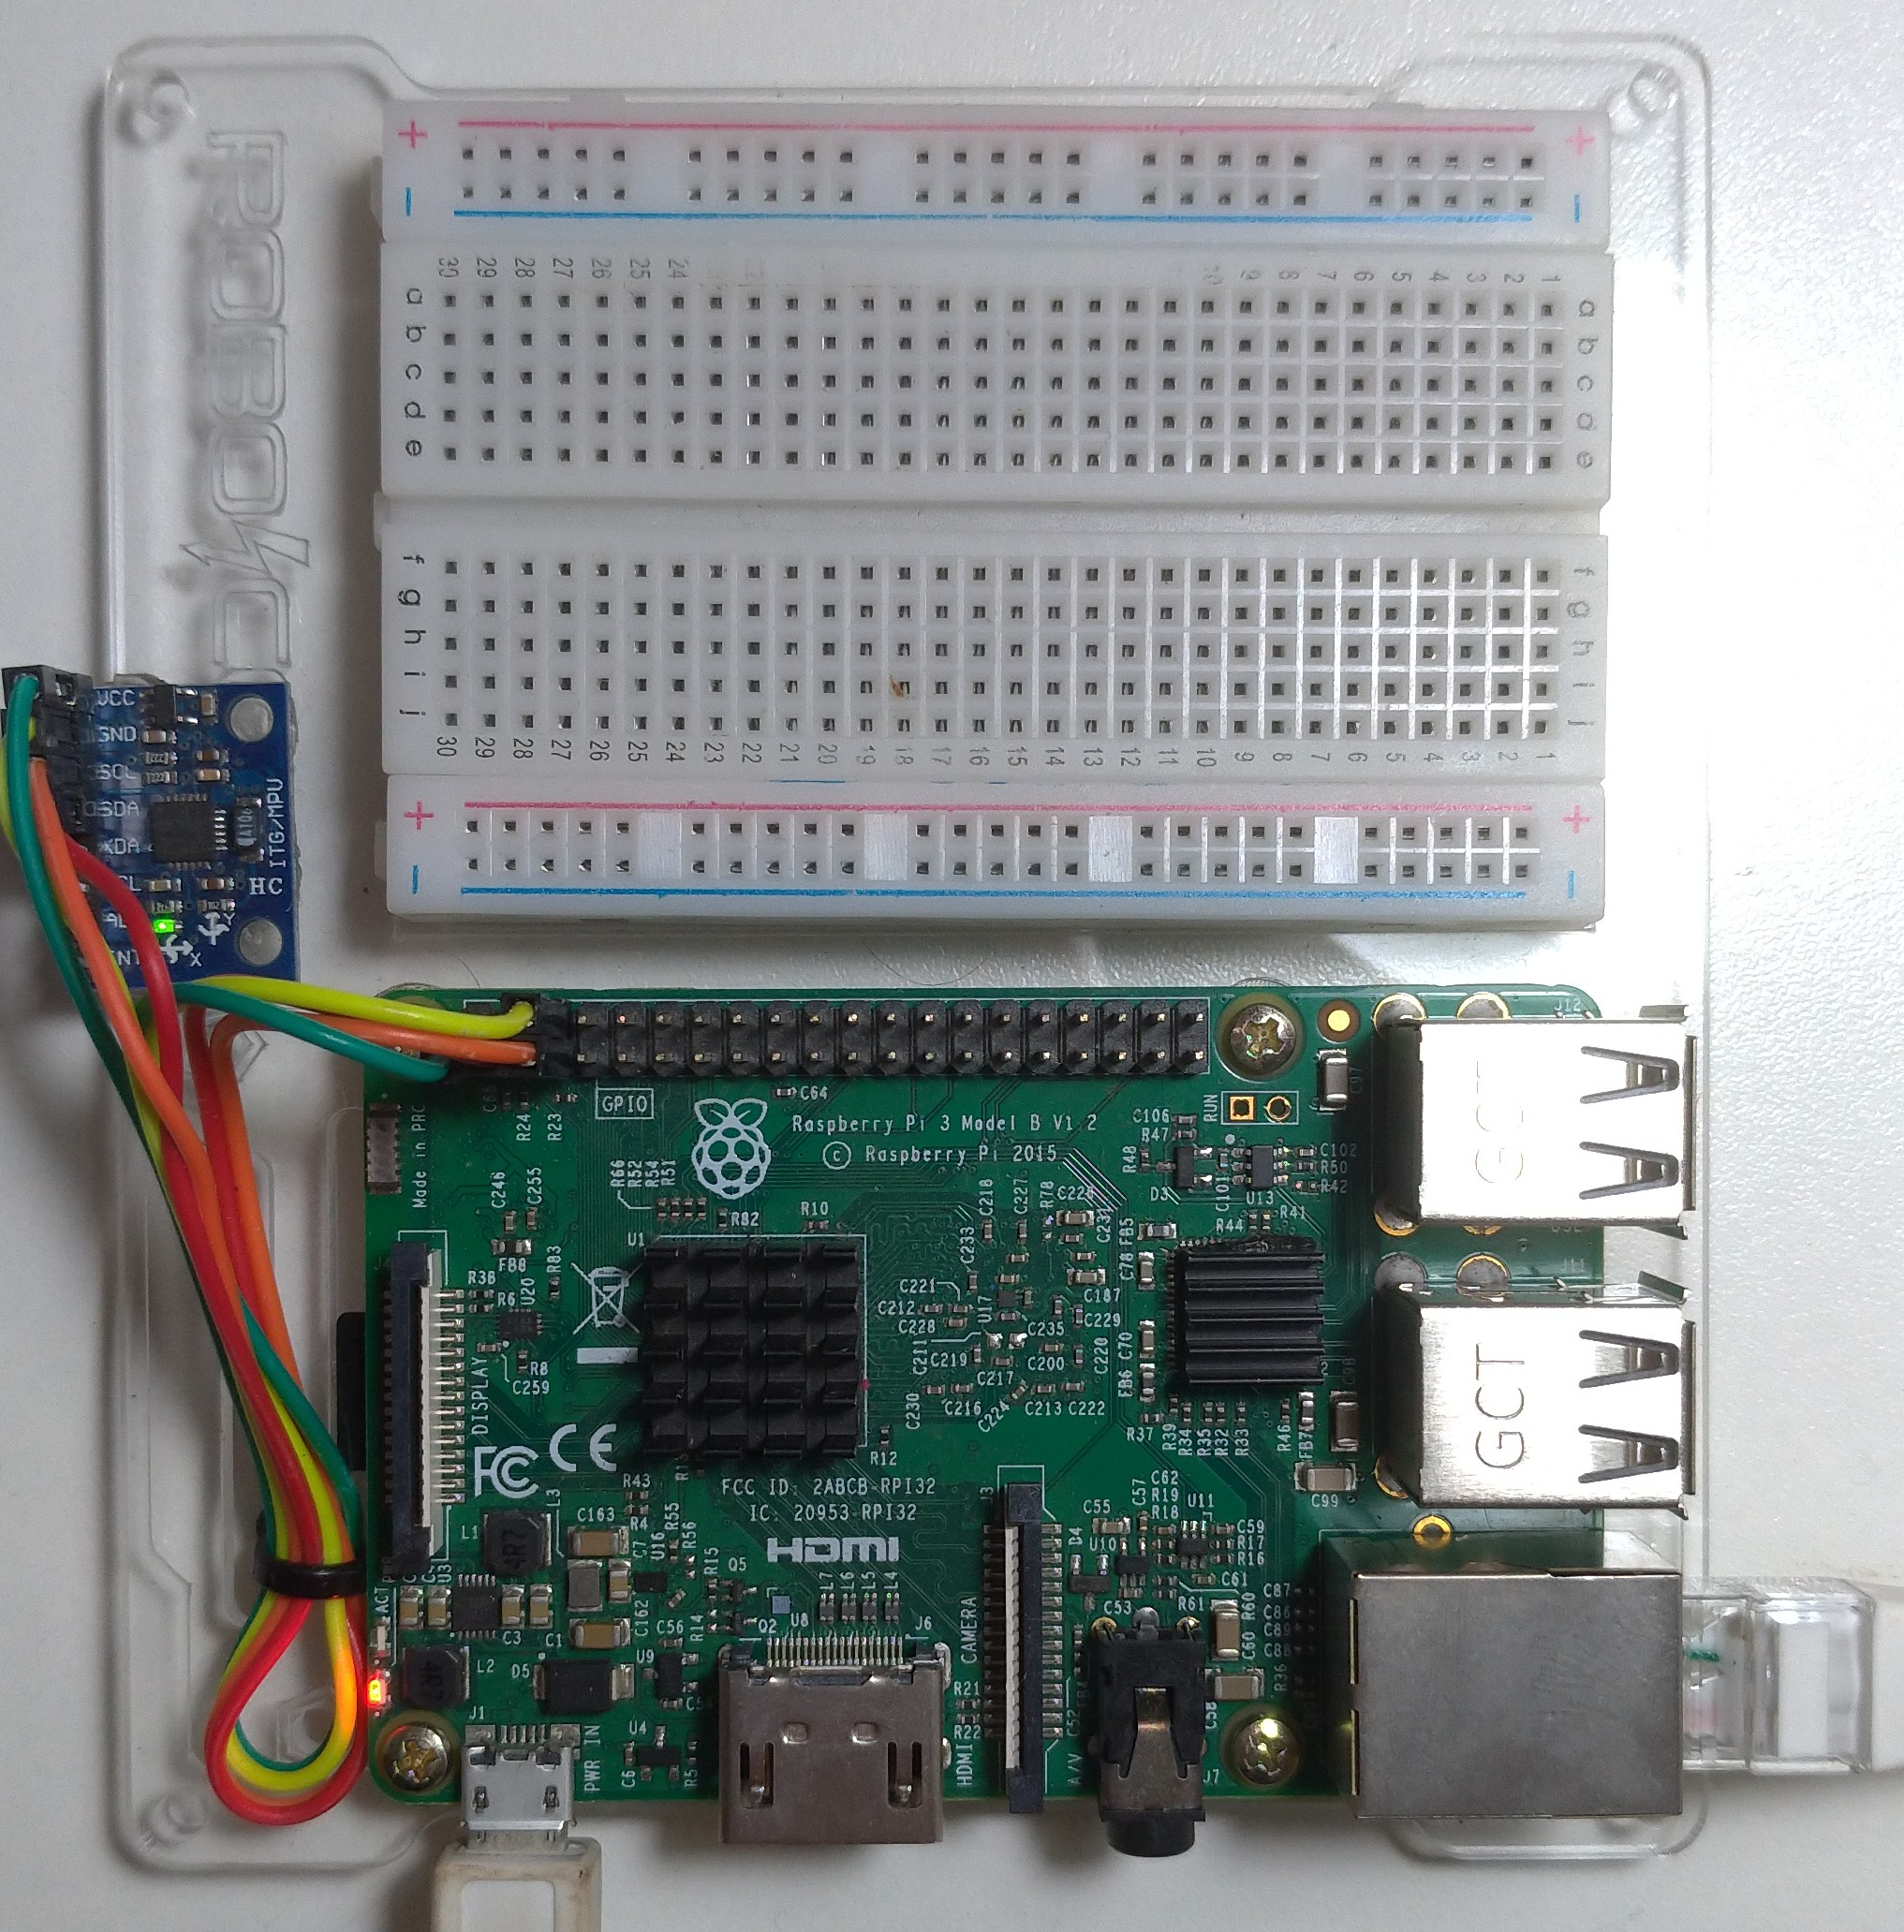
\includegraphics[width=0.5\textwidth]{figuras/mpu6050-proto-top.jpg}
    \fonte{o autor}
\end{figure}
